\documentclass[fleqn]{article}
\usepackage{tikz,tcolorbox}
\usepackage{array} % For customizing tables
\usepackage{booktabs} % For better horizontal lines
\usepackage[a4paper, paperwidth=25cm, paperheight=25.5cm, left=2cm, right=2cm, top=2cm, bottom=2cm]{geometry}
\usepackage{multicol}
\usepackage{amsmath}
\usepackage{pgfplots}

\pgfplotsset{compat=1.18}
\usepackage{makecell}
\usetikzlibrary{patterns}
\definecolor{greenPlot}{HTML}{14C877}
\definecolor{orangePlot}{HTML}{EA6E12}
\definecolor{purplePlot}{HTML}{4C12EA}
\definecolor{blueArea}{HTML}{10D9EE}
\definecolor{redPlot}{HTML}{F3490E}
\definecolor{myblue}{HTML}{338AC7}
\definecolor{p}{HTML}{D813E7}
\definecolor{y}{HTML}{F5F806}
\usepackage{amssymb}
\setlength{\parindent}{0pt}
\setcellgapes{3pt}  % Adjust padding as needed
\makegapedcells
\tcbuselibrary{skins, breakable, theorems}
\usepackage{algorithm}
\usepackage{algpseudocode}
\usepackage{xcolor}
\setlength{\mathindent}{8cm}
\renewcommand{\thealgorithm}{}
\definecolor{mypur}{HTML}{A938E1}
\newtcolorbox{prettyBox}[2]{
  enhanced,
  colback=white!90!#2,   % Background color based on the second parameter (color)
  colframe=#2!60!black,  % Frame color based on the second parameter (color)
  coltitle=white,        % Title color (white)
  fonttitle=\bfseries\Large,
  title=#1,              % Title from the first parameter
  boxrule=1mm,
  arc=0.5mm,
  drop shadow=#2!35!gray, % Drop shadow color based on the second parameter (color)
}


\usepackage{listings}
% Define the style for C code
\lstdefinestyle{cstyle}{
    language=C,
    basicstyle=\ttfamily\small,
    keywordstyle=\color{blue}\bfseries,
    stringstyle=\color{red},
    commentstyle=\color{green!50!black}\itshape,
    numbers=left,
    numberstyle=\tiny\color{gray},
    stepnumber=1,
    breaklines=true,
    frame=tb,
    tabsize=4,
    showstringspaces=false,
    captionpos=b
}



\newcommand{\exer}[1]{
  \section*{Exercice #1}
  \vspace{-0.5cm}
  \noindent\rule{\textwidth}{0.5pt}%
}

\newcommand{\tit}[1]{
\begin{center}
    \Large{\textbf{{#1}}}
\end{center}
}


\begin{document}

\renewcommand{\arrayrulewidth}{0.75mm} % Set line thickness

\setlength{\tabcolsep}{5.5pt} % Set horizontal padding

\renewcommand{\arraystretch}{1.5} % Set vertical padding (1.0 is default)


\tit{DW 3}



\begin{prettyBox}{Reminder}{greenPlot}
\textbf{Frequent Mistakes With Pipes}
\begin{itemize}
    \item \textbf{Closing All Read Descriptors Then Trying To Write On Pipe}: 
    Kernel doesn't find where to write the data, causing a SIGPIPE signal or an EPIPE error.
    \item \textbf{Not Closing All Write Descriptors Then Trying To Read From That Pipe}: 
    Kernel waits for the pipe to be written to, as it doesn't see an EOF (End Of File) signal.
\end{itemize}

\textbf{Solution}
\begin{itemize}
    \item \textbf{Leave at least one read end of the pipe open before writing to it}, 
    so the kernel knows where to write the data.
    \item \textbf{Always close all write ends of a pipe before reading from it}, 
    so the kernel knows that the pipe has reached its EOF.
\end{itemize}

\end{prettyBox}
\exer{1}

The goal of this exercise:

\begin{itemize}
    \item \textbf{child\_1}: Accepts input of n characters. Write only alphabetic characters to the pipe, converts lowercase letters to uppercase. Stops when the user inputs '0'.
    \item \textbf{child\_2}: Prints the characters written to the pipe by \textbf{child\_1}.
    \item \textbf{parent}: Creates the child processes and waits for them to finish.
\end{itemize}


\vspace{0.75cm}

The includes needed
\begin{itemize}
    \item stdio.h : to printf and get user input
    \item stdlib.h : to use exit to terminate whole 
programe and to terminate child process
    \item unistd.h :to use fork and pipe primitive
    \item ctype.h : to use toupper function
    \item sys/wait.h : to use wait primitive (parent wait for child to terminate)
\end{itemize}
\newpage
\lstinputlisting[style=cstyle,basicstyle=\footnotesize\ttfamily]{Questions/EX1/ex1Overview.c}

child\_1 void function :
\lstinputlisting[style=cstyle,firstline=10,lastline=33,basicstyle=\footnotesize\ttfamily]{Questions/EX1/ex1.c}

\vspace{0.5cm}

child\_2 void function :
\lstinputlisting[style=cstyle,firstline=36,lastline=50,basicstyle=\footnotesize\ttfamily]{Questions/EX1/ex1.c}



\begin{center}
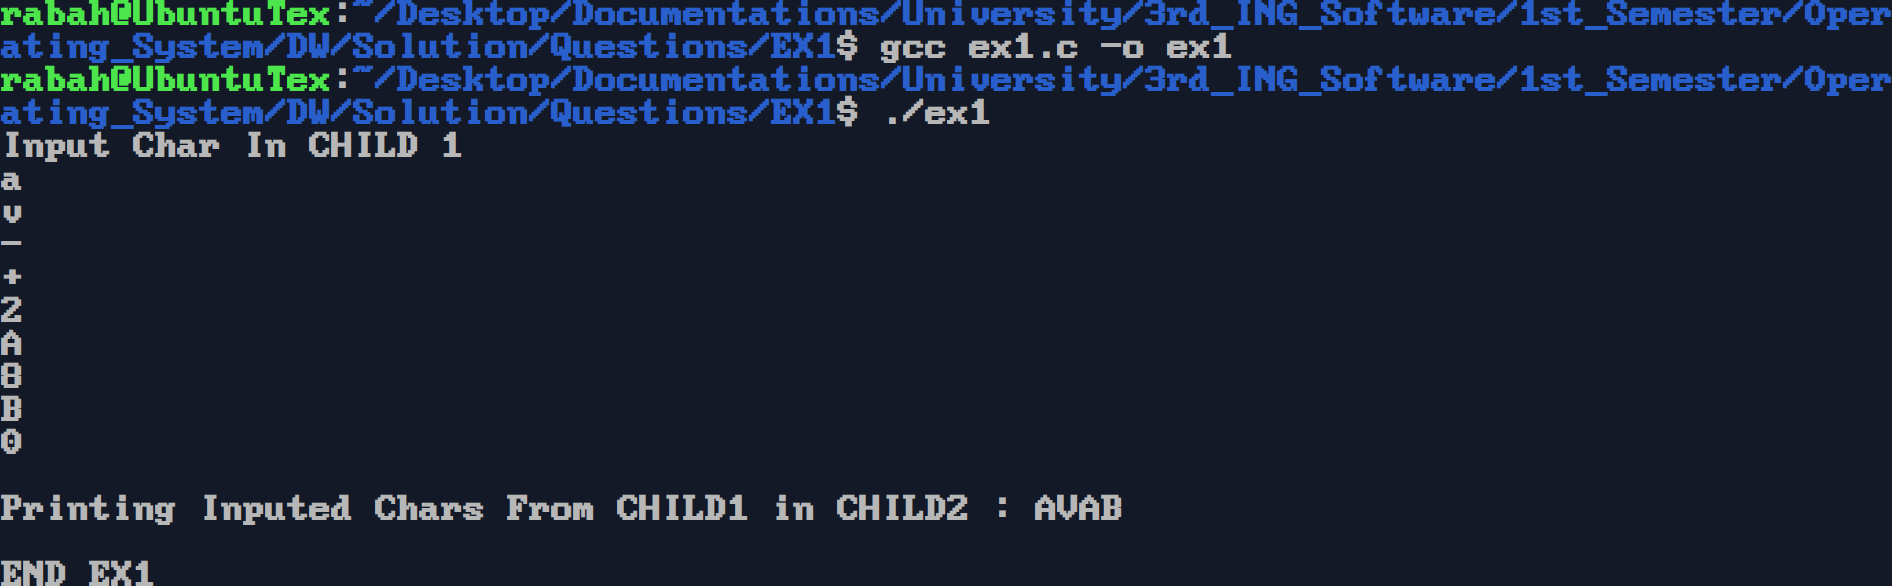
\includegraphics[width=\textwidth]{Questions/EX1/output.png}
\end{center}



\end{document}
